\documentclass[a4paper,11pt]{article}
\usepackage[pdftex]{graphicx}
\usepackage{lscape}

%\usepackage{draftwatermark}
%\SetWatermarkScale{5.0}

%
\vfuzz2pt % Don't report over-full v-boxes if over-edge is small
\hfuzz2pt % Don't report over-full h-boxes if over-edge is small

\setlength{\oddsidemargin}{0cm}
\setlength{\evensidemargin}{0cm}
\setlength{\textwidth}{16cm}
\setlength{\textheight}{24cm}
\setlength{\topmargin}{-1cm}

\begin{document}
\thispagestyle{empty}

% Common EURACE Title Page
% EURACE and FW6 logos
\vspace{\baselineskip}

\includegraphics[width=45mm]{EURACE-logo.png}		
\hfill

\includegraphics[width=45mm]{FW6-logo.png}

% Title
\begin{center}
Project no.\\
035086\\
Project acronym\\
{\bf EURACE}\\
Project title\\
{\bf An Agent-Based software platform for European economic policy design with heterogeneous interacting agents: new insights from a bottom up approach to economic modelling and simulation}\\
\end{center}

\vspace*{\baselineskip}\noindent
Instrument: STREP\\[\baselineskip]
Thematic Priority: IST FET PROACTIVE INITIATIVE ``SIMULATING EMERGENT PROPERTIES IN COMPLEX SYSTEMS\\

% Deliverable information: title & number
%\vspace*{2\baselineskip}
\begin{center}
{\bf
Deliverable reference number and title\bigskip\\
%D1.4: Porting of agent models to parallel computers\\
D8.4: Porting of the software platform to parallel computers
}\bigskip\\
Due date of deliverable:
%31/08/2008\\
31/08/2009\\
Actual submission date:
%30/09/2008\\
30/09/2009\\
\end{center}


% Project Info
\vspace*{\baselineskip}\noindent
{Start date of project: September 1$^{st}$} 2006 \hfill {Duration: 39 months}\\

%Deliverable Info - partner
\vspace{2\baselineskip}\noindent
Organisation name of lead contractor for this deliverable\\
{\bf STFC Rutherford Appleton Laboratory - STFC}
\begin{flushright} 
Draft
\end{flushright}

\vspace{\baselineskip}
\begin{table}[hb]
\begin{tabular}{||c|l|l||} \hline\hline
\multicolumn{3}{||l||}{\small Project co-funded by the European Commission within the Sixth Framework Programme (2002-2006)}\\ \hline
\multicolumn{3}{||l||}{\bf Dissemination Level}\\ \hline
\bf PU &\small Public\hfill~& \bf X \\ \hline
\bf PP &\small Restricted to other programme participants (including the Commission Services)& \\ \hline 
\bf RE &\small Restricted to a group specified by the consortium (including the Commission Services)&  \\ \hline
\bf CO &\small Confidential, only for members of the consortium (including the Commission Services)&  \\ \hline \hline
\end{tabular}
\end{table}
\pagebreak
% End of EURACE Title Page

\pagenumbering{roman}
% Table of Contents
\tableofcontents
\pagebreak

% Abstract/Summary
\begin{abstract}\noindent
Making use of high performance computers in agent-based simulation is a complex and difficult task. This report describes the approach being explored within the EURACE project to exploit parallel computing technology in large-scale agent-based simulations involving millions of agents. The underlying software is the FLAME framework and the report will give an overview of the features and use of FLAME and discuss the implementation of techniques that attempt to exploit large parallel computing systems.  

This report updates the ealier deliverable on porting FLAME to parallel systems - Deliverable D1.4 - and presents the developments of FLAME and the porting of the Full Integrated EURACE Model during the final year of the project.

Some of the initial results from the initial benchmarking activities have been included in the Appendix so as to provide a complete record of the FLAME developments.

In the first report the results presented demonstrated that the parallel implementation of FLAME worked and is portable between a number of systems the efficiency is quite poor as the full implementation of message filtering is not yet complete and filtering is not yet fully exploited within the EURACE models. During the
final year significant developments have been made to FLAME and the underlying Message Board Library that significantly improved both its serial and parallel performance. The filtering available within FLAME has been enriched and its utilisation within the framework improved. 

The report presents the developments of FLAME and its associated analysis tools during the final period which including a model consistency check, a initial validation tool and various static and dynamic analysis tools to help the assessment of model performance.

The final section of the report describes the results achieved in benchmarking the EURACE Model at the time of writing. Although largist populations can be simulated - in the order of 30,000 agents - we have not been able to achieve the 100,000s that was the potential goal of the project.
\end{abstract}
\pagebreak
\pagenumbering{arabic}

% Start of document
%
% Fix page number

%
% General structure
%   1. Introduction
%   2. Characterisatics of Agent Based Simulators
%   3. General Parallel Implementation of FLAME.
%   4. Detailed Desciption of Parallelisation
%   5. Detail on Dynamic Load Balancing
%   6. Testing: Functional and Portability
%   7. Benchmark Problems
%   8. Future Development and Optimisation
%   9. Conclusion\section{Introduction}
\section{Introduction}	In this deliverable we present the internal logical consistency of the fully integrated EURACE model.
Since the focus of WP8 is on the development, integration and validation of the EURACE model, we found it appropriate to restrict D8.5 to these topics. This deliverable therefore does not contain any scenarios or policy experiments, which are collected in WP9.

Chapter 1 describes the construction of a system of national accounts for EURACE, with all the interlinkages between the balance sheets of the agents. We provide a set of accounting rules that should be satisfied for the model to be stock-flow consistent. We have verified that all these rules a true for the fully integrated model, thereby validating the internal logical consistency of all monetary and physical flows.

Chapter 2 on robustness checks shows that the model is robust against changes in critical model parameters and to scaling of the population size. We also show the effects of synchronous versus asynchronous timing of the agents.

Finally, in Chapter 3 we show benchmark results for the Integrated Model that provide the background for the more elaborate policy experiments presented in D9.1-D9.3. 
\section{General Parallel Implementation of FLAME} The FLAME architecture has some inherently good characteristics that lend itself to parallelisation. Unfortunately, it also has a number of bad characteristics. Because FLAME is an application generator
it does not have a full understanding of the application it is generating. Agent-based applications could be characterised as a set of communicating tasks. Although the agent population and their interactions can be specified \textit{a priori} the computational load of each agent and the number of communications they perform are very difficult to determine without running the code. 

We will not address the dynamic re-configuring of an agent population at run time. Initial experiments have shown that this is a very complex problem where there are many trade offs to be considered. In this effort to have an automatically generated parallel implementation of a FLAME application we focus on the most basic characteristic of FLAME and its agents: that of communications - agent to agent. This communication between agents is implemented within FLAME as a set of \textit{message boards} on which agents post messages (information) and from which agents can read the messages (information). There is one message board per message type and FLAME manages all the users interactions with the message boards through a Message Board API.

In a fully connected and communicating agent population, interaction may not be local but long range leading to many-to-many, inter-node communication which can drastically impact the scalability and simulation time. However, in many applications of FLAME, we have seen that there is sufficient locality (that can be taken advantage of) to consider parallelisation taking into account the general population sizes. 

The use of simple read/write, single-type message boards allows the framework implementer to divide the agent population and their associated communications areas. This division could be based on any number of parameters or separators but the simplest to appreciate is position or locality. If, as in EURACE, agents are people or companies for example, they will have locality defined either as location or by some group topology. It is also reasonable to assume that the dominant communications in both scenarios will be with neighbouring agents.

As explained above, FLAME uses a collection of message boards to facilitate inter-agent communication. As the majority of large high performance computing systems currently use a distributed memory model a Single Program Multiple Data (SPMD) paradigm is considered most appropriate for the FLAME architecture. The parallelisation of FLAME utilises partitioned agent populations and distributed message boards linked through MPI communication. Figure~\ref{fig:Figure2} shows the difference between the serial and parallel implementation.

\begin{figure}[h]
	\centering
		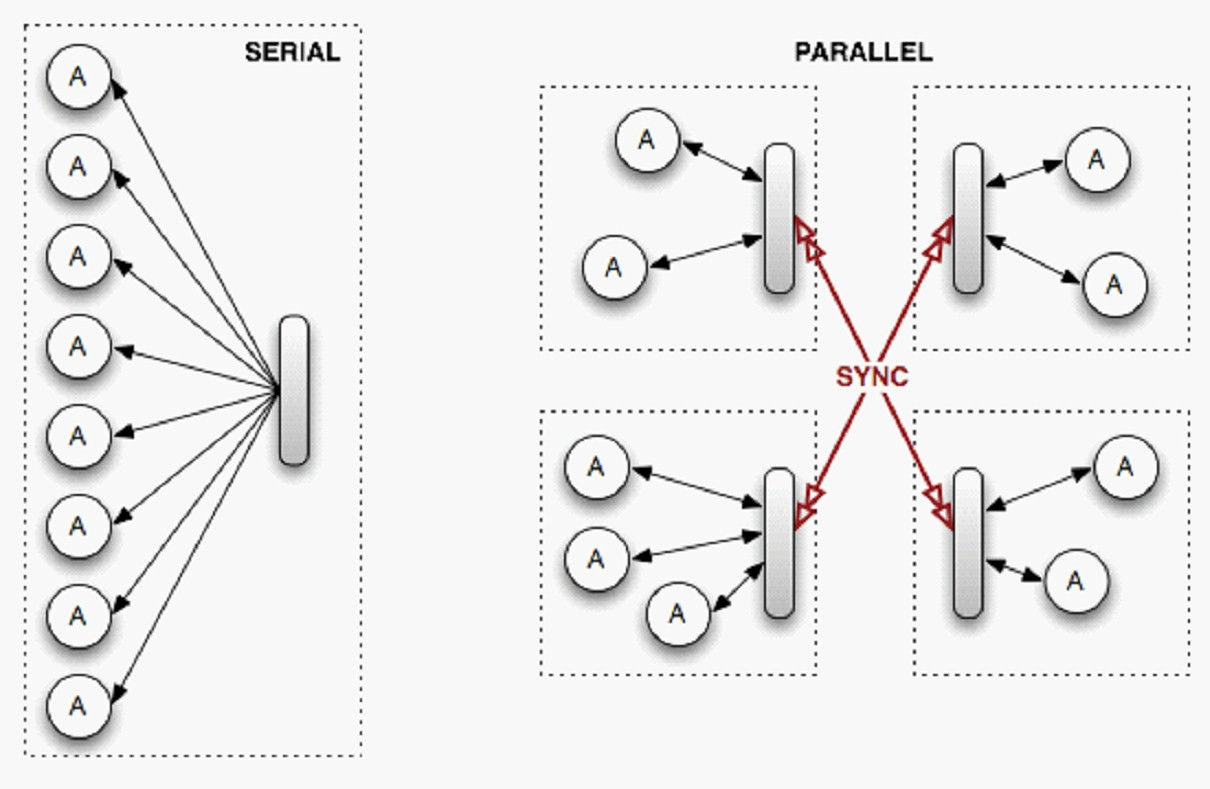
\includegraphics[scale=0.25]{flame.jpg}
	\caption{Serial and Parallel Message Boards}
	\label{fig:Figure2}
\end{figure}

The most significant operation in the parallel implementation is providing the message information required by agents on one node of the processor array but stored on a remote node of the processor. The FLAME Message Board Library manages these data requests by using a set of predefined message filters to limit the message movement. This process could be considered a synchronisation of the local message boards within an iteration of the simulation. This synchronisation essentially ensures that local agents have the message information they need as the simulation progresses.

An additional advantage of implementing parallelism in FLAME through the Message Board Library is that development of the FLAME framework and the message board algorithms can continue independently to a great extend as the Message Board API defines the interface between the two elements of the code. This should enable the message board routines to be developed and optimised without major re-engineering of the framework.

The two main areas of algorithmic and technical development needed to achieve an effective parallel implementation are load balancing and communications strategy. 

Initial load balancing is not too difficult: we have a population of agents, of various complexities, to which we can assign relative weights and so in the most general case the agents can be distributed over the available processors using the weights. This may well give an initial load balance but makes no reference to the possible communication patterns of the agent population. As the simulation develops the numbers of agents in the population may change and adversely affect the load balance of the processors. It is a very interesting and difficult problem to gauge whether the additional work (computation and communication) involved in remedying a load imbalance  is worth the gain. Given that the goal of any dynamic re-organising of the agents is to reduce the elapsed time of the overall simulation, determining whether a process of dynamically re-balancing the population will contribute to this is very problematic. It may well be that a slight load in-balance will have no significant effect of the wall clock time of the simulation. These problems are under investigation.

The patterns and volumes of communication for the population will have a considerable impact on the performance and parallel efficiency of the simulation. In general, agents are rather light-weight in terms of computational load. Where all agents can and do communicate with all others the communications load within and across processors will be great. Fortunately communications within a processor are generally efficient. However across processors this communication can dominate the application. Within FLAME communication between agents is managed by the Message Board Library, which uses MPI to communicate between processors. The Message Board Library implementation attempts to minimise this communication overhead by overlapping the computational load of the agents with the communication. 

Where the agents have some form of locality the initial distribution of agents makes use of this information in placing agents on processing nodes. During the simulation agents can be dynamically re-distributed to maintain computational load balance. However given the light-weight computational nature of many agent types the effect of dynamically re-distributing agents on the grounds of their communications load may well turn out to be more important than considering computational load.

Within the EURACE Project a parallel version of FLAME has been developed using these ideas and the sections below discuss some of the results in performing parallel simulations.


\section{Detailed Description of Parallelisation} % BEGIN (PARALLELISATION)
% ===========================================================================
\subsection{Overview}

Within a FLAME simulation, every agent only interacts with its environment via the reading and writing of messages to a collection of Message Boards. This makes the Message Board component an ideal candidate for enabling parallelism. 

Using distributable Message Boards, agents can be farmed out across multiple processing nodes and simulated in parallel while coherency of the simulation is maintained through the unified view of the distributed Boards.

\begin{figure}[h]
 \centering
  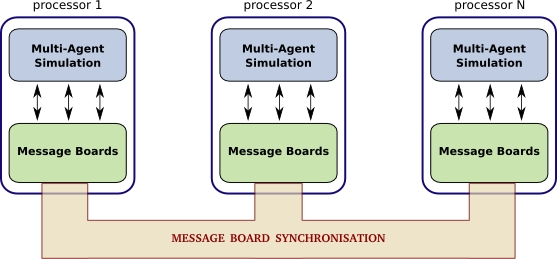
\includegraphics[scale=0.50]{mboard_flame.jpg}
 \caption{Parallelisation of FLAME using distributed Message Boards}
 \label{fig:mb_flame}
\end{figure}

\subsection{The Message Board library}
In the recent code release, the Message Board was decoupled from the FLAME framework and implemented as a separate library. This provides us with the flexibility to experiment with different parallelisation strategies while minimising the impact on current users of the FLAME framework.

\begin{figure}[h]
 \centering
  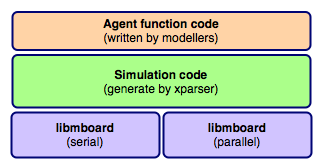
\includegraphics[scale=0.60]{mboard_overview.png}
 \caption{Users can create either serial or parallel executables by linking their object files to the appropriate \textit{libmboard} library}
 \label{fig:mb_overview}
\end{figure}

The Message Board Library (\textit{libmboard}) was built as a set of static libraries which can be linked to users' simulation object files to create serial and parallel executables. This setup enables users to maintain a common source base for both serial and parallel simulations, thus simplifying code management and testing. It will also provide \textit{libmboard} developers the facility to quickly switch between different library implementations without having to continuously recompile the test program.

All functionality provided by the Message Board Library is accessible via the \textit{libmboard} Application Program Interface (API). This is discussed further in Section~\ref{sec:mb_api}.

Within the FLAME framework, the \textit{libmboard} API is used within routines generated by the framework and not directly by the modellers. Modellers are provided with model-specific routines that hides to complexity of managing boards and packaging data into suitable datatypes. Figure~\ref{fig:mb_api_flame} provides and example of this whereby an agent's message add request gets translated to a \textit{libmboard} API call.
\begin{figure}[h]
 \centering
  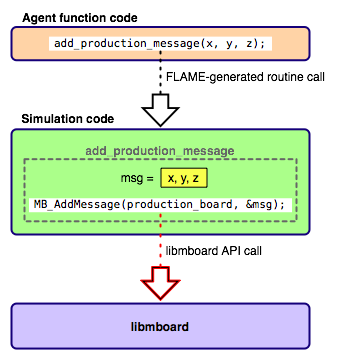
\includegraphics[scale=0.60]{mboard_codetranslate.png}
 \caption{Modellers use FLAME-generated routines which gets translated to the appropriate \textit{libmboard} API call}
 \label{fig:mb_api_flame}
\end{figure}

\textit{libmboard} uses MPI to communicate between processors, and POSIX threads (pthreads) to manage a separate thread for handling data management and inter-process communication. Futher details are available in Section~\ref{sec:mb_sync} and Section~\ref{sec:commthread}.

% ===========================================================================
\subsection{The \textit{libmboard} API}
\label{sec:mb_api}

\begin{itemize}
\item Quick desc of the API. Point to User Doc for details.
\item Opaque objects
\item return codes
\end{itemize} 


% ---------------------------------------------------------------------------
\subsubsection{Library environment}

\begin{itemize}
\item Init and finalise
\item MPI env
\item fork/join comm thread thread
\end{itemize} 

% ---------------------------------------------------------------------------
\subsubsection{Boards}

\begin{itemize}
\item create/clear/delete
\item AddMessage.. clone mem vs storing ptr
\end{itemize} 

% ---------------------------------------------------------------------------
\subsubsection{Iterators}

\begin{itemize}
\item isolate users from internal data representation
\item normal/filtered/sorted
\item returning cloned mem vs ptr.
\item randomisation
\item rewind
\end{itemize} 

% ---------------------------------------------------------------------------
\subsubsection{Synchronisation}
\label{sec:mb_sync}

\begin{itemize}
\item Message Tagging vs Filtered Iterators.
\item Why important? Impact on solution time?
\item Details on how messages are packed and distributed
\end{itemize} 

\begin{figure}[h]
 \centering
  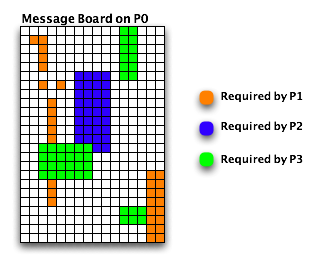
\includegraphics[scale=0.70]{taggedboard.png}
 \caption{Lorem ipsum dolor sit}
 \label{fig:taggedboard}
\end{figure}

When synchronisation of a board is requested, the board is locked and added into the \textit{Sync Queue}. Control is then returned to the the calling code, allowing it to perform other tasks that does not require access to the board being synchronised. 

The sequence diagram in  Figure~\ref{fig:syncboard} depicts how ra board synchronisation request may take place. The process of actually synchronising and unlocking the board is performed concurrently in the background by the \textit{Communication Thread}. This is discussed further in Section~\ref{sec:commthread}.

\begin{figure}[h]
 \centering
  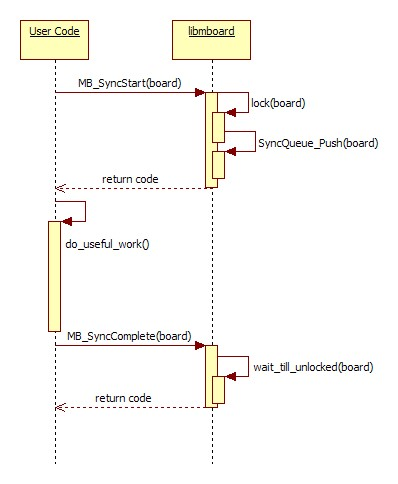
\includegraphics[scale=0.60]{syncboard.jpg}
 \caption{Other work can be schedule during board synchronisation to shadow the overheads of communication}
 \label{fig:syncboard}
\end{figure}

% ===========================================================================
\subsection{The Communication Thread}
\label{sec:commthread}

During the initialisation of the Message Board environment, \textit{libmboard} forks a \textit{Communication Thread} to handle the synchronisation of distributed boards. 

Apart from potentially making better use of multi-core processors, delegating communication and memory intensive operations to a separate thread also allows us to minimise the effective overheads by performing them concurrently with the main simulation and thus overlapping the Board synchronisation time with that of useful computation.

To simplify thread-safety, the \textit{Communication Thread} interacts with the main thread mainly through the \textit{Sync Queue} and the locking mechanism of each board. Access to these components are protected by mutex locks provided by \textit{pthreads} API. Boards that need to be synchronised are locked by the main thread and pushed into the \textit{Sync Queue}. The \textit{Communication Thread} indicate the completion of a synchronisation process by unlocking the board.

\begin{itemize}
\item motivation
\item queues
\item state diagram
\end{itemize} 



\begin{figure}[h]
 \centering
  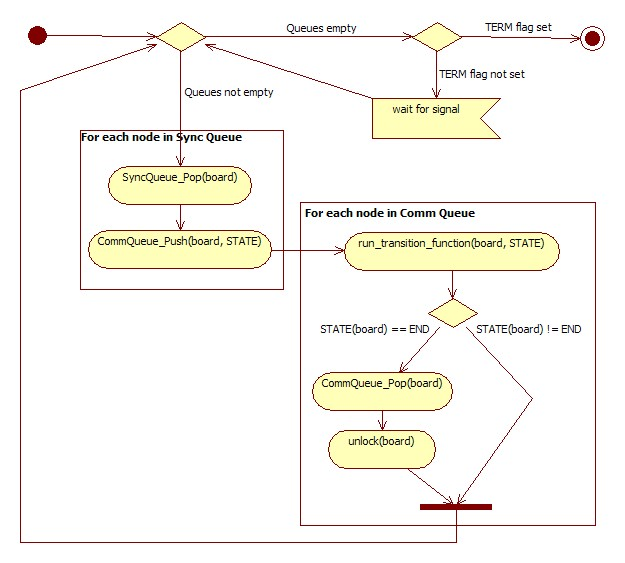
\includegraphics[scale=0.50]{commloop.jpg}
 \caption{Activity diagram for Communication Thread}
 \label{fig:commloop}
\end{figure}

\begin{figure}[h]
 \centering
  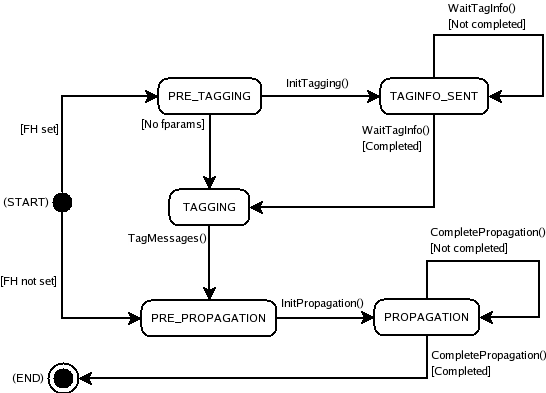
\includegraphics[scale=0.50]{CommNode.png}
 \caption{State diagram for processing Communication Node}
 \label{fig:commstate}
\end{figure}

% ===========================================================================
\subsection{Issues}

\begin{itemize}
\item MPI thread support
\item MPI sends/receives requires contiguous buffers. Expensive (space and time) packing of messages.
\item Comm stages not fully non-blocking
\item Total tagged messages may be more than actual message. Gets works with more proc. Scaling issues.
\end{itemize} 

% ===========================================================================

\section{Initial Data Partitioning} \subsection{Introduction}

As described above in general terms parallelisation in FLAME has been introduced through distributed message boards and distributed agents populations. Hence at the start of any simulation the agent population must be distributed over the available processors.

As achieving some form of load balance - each processor performing a similar work load - is important in reducing the elapsed time of a simulation, the initial distribution of the population should attempt to achieve this. However such an initial distribution can only be based on the information provided in the XMML models files and the associated user provided C code. In the current version of FLAME there is little useful information provided.

Although achieving a load balance over the processors is important in reducing elapsed time reducing inter-processor communication is equally if not more important in agent-based applications. Deriving information on the communications load of an agent population can only be achieved whilst the application is executing although some information can be derived from the XML and C code.

Two basic methods of static partitioning have been developed: partitioning based on a separator and \textsl{round robin} partitioning.

\subsection{Separator Partitioning}

Separator partitioning distributes the agents amongst the partitions based on one or more memory variables of the agent. Every agent must have these variables for this to work and the variables can be either discrete or continuous numerical values. The most obvious example is distributing agents using their position ($x,y, z$ co-ordinates) which gives a good initial distribution in cases where communication is between near neighbours. This is already implemented in FLAME due to the frameworks initial field of application, biological systems, and is referred to as \textit{geometric partitioning}. 

Other examples of separators could be region or country id, but the overall aim is to get those agents that will generate a lot of communication with each other on to the same partition - something that is not always feasible.

\subsection{Round Robin Partitioning}

This is the simplest form of partitioning in which agents are distributed, one at a time to each partition in turn. No account is taken of behaviour during the simulation but this may be the only way of partitioning if the agents have no common memory variables. This type of partitioning is implemented in FLAME.

It is possible to extend this method by using the agent type as a discriminator. Agents of a particular type would be allocated to one partition (or a set of partitions) on a round robin basis if it were known (or envisaged) that agents communicated with other agents of their own type more than any other type. (This could also be seen as a special form of separator partitioning.)

\subsection{Other Benefits}

As well as hoping to improve the load balance, partitioning of the initial data will mean that each node in the compute system will have to read only its data. In the current version of FLAME one node has to read all the data, decide on the partitioning and then distribute the data with which agents can be partitioned. Then all the nodes have to read all the initial data picking out only those agents that fall within their partition.



\section{Initial Data Generation} \subsection{Introduction on Cloning}

As the EURACE model became more and more complicated so did the relationships between agents. These realtionships are both inter- and instra- regional and provide a complex set of constraints for the initial population of agents. As modellers and computer scientists demanded larger populations it was found that the Tubitak population GUI could not provide populations quickly enough and ran into memory problems even on very well specified machines. For this reason a simpler method of creating large populations was designed, that of \textit{cloning} one population many times replacing agent ids as required.

A variety of implementations were tried, \texttt{bash} scripts using \texttt{sed/awk}, python code and finally and most successfully C code that could run in serial or in parallel. The seed population for cloning has one region and so there are intially no inter-regional interactions but it is possible for these to occur in the transient stage of the simulation if the model is set up correctly. The lack of these interactions means that cloning is a perfectly parallel algorithm.

Cloning from a single region also has the benefit that it is possible to provide pre-partitioned input data for the parallel implementation of the EURACE model. For example, clone one region to give 16 regions and input files for 1, 2, 4, 8 and 16 processes can be easily produced.

The cloning process relies on a special \texttt{xml} file in which any agent ids are marked with \texttt{REPLACE\_ID\_n} where \texttt{n} is the id of the agent in the region being cloned. This \texttt{xml} file is produced from a \texttt{pop} file by the \texttt{instantiate.py} script written by Tubitak and using code from the population GUI. The script is invoked as

\begin{verbatim}
python instantiate.py -r 0_bench_oct_12.pop 0_markers_oct_12.xml
\end{verbatim}

Actually cloning the region is illustrated by the following example:

\begin{verbatim}
./clone.sh 0_markers_oct_12.xml 8 tmp -r 2
\end{verbatim}

This clones \texttt{0\_markers\_oct\_12.xml} creating 2 input files each containing 8 regions. The output files are put into a directory called \texttt{16R\_2P} indicating that this is input for a 16 region run on 2 processes.

It is possible to control which agents are cloned by listing their names in the file \texttt{agent\_list.txt}.

\subsection{Implementation of Cloning}

The cloning application runs from the commandline using a \texttt{bash} script to control the cloning and organisation of output files, \texttt{sed} to perform some ad-hoc text manipulation of output files and a C application to do the computationaly intensive work of reading the input file and writing an output file. Both serial and parallel (MPI) versions of the C code are available.

The serial code works by repeatedly calling it with arguments that are the increment to make in id numbers between regions and a number (0 based) of this particular clone. The id increment is set to the number of agents in the original region since there can be no more agents in any cloned region. Running the code in paralle requires only the increment value to be given as each process can get the clone number as its node id by calling \texttt{MPI\_Comm\_rank}.

{\raggedright Source code is available from the EURACE Subversion repository \break \verb+http://ccpforge.cse.rl.ac.uk/svn/eurace/models/utils/cloning+.}

\section{Job Submission with ExpGUI} %\subsection{Integration with Experimental GUI}
\subsection{The EURACE GUIs}
\subsection{Integration}
It was thought at first that the job submission bash shell scripts could be used by the experimental GUI for remote working, even on a Windows machine using Cygwin or MSYS. A later decision to make the Windows GUIs work natively meant that this could not happen and so an alternative implementation has been necessary. By making use of paramiko (\verb+http://www.lag.net/paramiko/+) and implementation of the SSH2 protocol for python, the remote execution and copying of files has been implemented to run natively on all platforms.  Scripts that run on the remote machine have been left as bash scripts as all the compute clusters run some version of Linux or Unix and the existing remote host configuration files can be used. 

At present from the experiment GUI the user can:

\begin{itemize}
\item choose the remote host
\item specify a serial or parallel job
\item specify the number of processes for a parallel job
\item run the job
\item check on job status (if remote system uses batch processing)
\item retrieve results.
\end{itemize}

Resource constraints have meant that it has not been possible to implement the full requirements of Projects containing Jobs within the experimental GUI.


\section{Tools for FLAME and Model Assessment} %\section{Tools for FLAME and Model Assessment}

\subsection{Static and Dynamic Analysis Tools}

EURACE has developed a very complex model in which there are many agents and many communications. The nested model directories contain 11 subdirectories and $\sim$50 XMML and C-code files. Checking the consistency of the model is a very difficult task. Although FLAME's parser will check the validity of $xml$ within the contex of the DDT of FLAME tags, checking that messages are used in a consistent way is difficult.


There are many elements to the testing and assessment of an application. This is the harder in the case of FLAME as FLAME is a program generator. The project has agreed development standards for all software developed which includes FLAME and any C code component of the EURACE Model. These are detailed in other reports and on the EURACE Wiki. We have not only to verify that FLAME generates \textit{correct} code as defined in the FLAME Model definition but also that the generated code is also \textit{correct}.


Although there is a Unit Testing suite for FLAME it is not for FLAME its targetare the FLAME model functions. It addresses the verification and consistency of agent function calls once the model has been parsed by the \texttt{xparser} using the model XMML files.

??????????????May be more here about Unit Testing


A number of static and dynamic analysis tools have been developed to perform these types of analyses. These tools include the following analyses:

\begin{description}

	\item [analyses\_mode.py]: a static analysis of the FLAME model which gives detailed information on the components of a model: agent, funtcion and messages types, number and sizes, a static communications table, a weighted communications table.

	\item [check\_message\_consistency.py]: a static consistency checker which compares the XMML definition with C code and ensures that the number and usage of messages is consistent.

	\item [The MM Package]: The \textit{MM} package is a dynamic to monitor message traffic in the simulation. It is a set additional directives included in the FLAME Templates which embedded in the application code that monitor all message traffic and outputs to an SQL data base. The data base can be post processed by the developed to assess the message traffic in the model. It also gathers information on the agent population in the simulation and the records of all function calls.

	\item [The Time Package]: The \textit{Timer} package described in Appendix \ref{timer} has been used to measure elapsed CPU time for functions and message board synchronisations. Knowing which functions take the longest time has helped to narrow the application of more detailed profiling tools such as \texttt{gprof} allowing for quicker identification of problems and possible solutions. Analysis of message board synchronisation times has shown that the message board implementation has provided excellent overlap of communication and computation.

\end{description}


\subsection {FLAME Verification}

Verification and validation of FLAME and its parallel implementation is again made difficult by its nature. We must verify and validation FLAME itself and we must also verify in some way the application generated by FLAME. It should be noted that FLAME has two distinct parts: the \texttt{xparser} which generates the application from the models XMML and C code files and \textit{The Message Board Library - libmboard} which is the underlying infrastructure that manages the inter-agent communications. \textit{libmboard} also provides an application to any parallel hardware through the MPI message passing interface.


\textit{libmboard} has is own set of unit tests and test programs. It has been developed using an agile test driven methodology.

?????????????????????More text????????????????????


The \texttt{xparser} has its own set of tests which are detailed in other reports.


For the developers we need to verify that FLAME is generating the model specified in the XMML and C code and that the execution of the generated application is \textit{correct}. Throughout the project we have gather a number of test examples which help verify the FLAME implementation. These test examples are model definitions and their associated C code. 


\subsection{Model Validation}

Validating the outputs of any simulation code generated by FLAME is in itself difficult. This will really require mining the outputs of the application and making comparisons with analytic or observer results.


\section{Performance of the FLAME Framework} The parallel implementation of FLAME seeks to use an SPMD paradyn - each node of the parallel system is running the essentially same $program$. However given the nature of agent-bsaed modelling and the FLAME implementation each nodal program could perform a very different sequence of instructions and function activations as it traverses its part of the state space. 

The two fundamental design features of FLAME is that all communications between agents takes place through a specified message board - a message respository - and that these message boards are distributed over the processing nodes of the parallel system. These message boards can be considered the data load and the agents themselves the computational load. In FLAME both these are distributed over the computational nodes.

However, although there may be some imbalance in computational load, with a reasonable initial data - agents - distribution, any imbalance should be small. The crucial element in the parallel implementation of FLAME is the distribution of the message boards over the system and their syncronisation.

Use Times Library to measure the wait time for each message board to complete syncronisation.


 
%\section{Remote Job Submission} %job submission
\subsection{Introduction}

A job submission system for FLAME jobs has been designed and implemented  so that it is easy to run EURACE on remote (parallel) machines. It will rely on the user knowing details of how to connect to the remote machine and details of the job scheduling software it uses. This data will be stored, in the appropriate format in a machine configuration file. The sequence of steps for job submission was drawn up in discussion with TUBITAK and is as follows:

\begin{enumerate}
 \item \textbf{Check authentication}. Does the user provided information allow a log in to the target machine? Return code for success/failure.
    \item \textbf{Check FLAME version}. Is the required version of FLAME available on the target machine? If not copy files onto target and install. Return code for success/failure of installation or success if installed. Could be some output text to say when FLAME has to be installed.
    \item \textbf{Create a project}. Send the model XMML file and C code. Parse and compile the model. Return code for parse failure/compilation failure/success. Success return code is the project id.
    \item \textbf{Submit job}. Send the 0.xml file(s) and project id. Submit the job according to data in the machine's configuration file. Return code code for success/failure. Success return code is the job id.
    \item \textbf{Query job status}. Send project and job id. Return code pending/done/running/failed.
    \item \textbf{Query status of all jobs in project}. Send project id. Return code is whether data is returned or not. Return text could be {job id, status} for each job.
    \item \textbf{Query status of all jobs in all projects}. Return code is whether data is returned or not. Return text could be {job id, status} for each job.
    \item \textbf{Get results}. Send project and job id. Copy results back and gather if parallel. Return code for success/failure. 
\end{enumerate}

The details for each of these steps are given later.

Connection to remote machines will be via \texttt{ssh} a standard secure connection mechanism which encrypts data between machines, or \texttt{gsissh} a grid-enabled version of ssh (part of Globus \verb+http://www.globus.org+) which requires the user to have a grid (X.509) certificate. The scripts will work best if the user arranges for login authentication without a password. For ssh this means generating a public/private key pair (see the Authentication section of \texttt{ssh} manual and the \texttt{ssh-keygen} manual for details). The public key should be copied to the remote machine and then, using \texttt{ssh-agent} as shown below the operations can be carried out without further authentication.

\begin{verbatim}
# Get the environment variables for ssh-agent
ssh-agent > file
# Set the variables
. ./file
# Add the private key to this session. Will require pass phrase for ssh key
ssh-add
# Run the job submission you want. As an example I have put in a simple ssh
ssh user@remote.machine.ac.uk
# Kill the ssh-agent session
ssh-agent -k	
\end{verbatim}


For gsissh the process is different. The local Grid computing community will have details on obtaining and using a Grid certificate and possibly be able to give advice on installing enough of Globus to use gsissh. It is beyond the scope of this document to go further.

\subsection{Authentication}

This will check whether the user and remote machine data given in the configuration file allow a log in to the remote machine. Comparing the hostname of the remote machine with that in the configuration file will indicate whether the log in was successful or not.

\subsection{Check FLAME}

Check for the xparser executable on the remote machine, assuming that its presence means that necessary libraries (such as the message board library) are therefore present. First look in the \texttt{\$PATH} environment variable and if not found then look in a known directory where a previous check may have installed the parser. If the parser is found then check the version against that version required by the user. If the version is correct the script finishes. 

If the parser is not found or the version is incorrect then the script copies the source for the parser and associated libraries to the remote machine and builds and installs them in a known directory.

\subsection{Create Project}

A project comprises the XMML file and C code for a model and then jobs are added to projects by giving the initial data, number of iterations and number of partitions for a FLAME run. The project is created by giving a directory on the local machine where the XMML and C code files can be found and they are copied to the remote machine. The xparser is run on the copied data and the resulting C code compiled. Errors from the parsing or compilation stages are reported where necessary and when the project has been successfully created it is given a project id that is returned to the user. 

\subsection{Submit Job}

The initial data file is copied to the remote machine and the run initiated for the user defined number of iterations and number of partitions. The job should be assigned to a particular project so the system knows what model is to be run.  Typically large parallel machines use some form of job scheduler to ensure users get a fair share of the machine and details of how to submit jobs to the scheduler should be provided by the user. These details go in the configuration file. When the job is scheduled on the remote machine the script returns a job id for the user to use later in queries.

It is possible to run jobs interactively, that is the script starts the job and waits until it is complete before returning.

\subsection{Query Job Status}

There are a number of variations for job status query, the simplest being querying the status of one job from one project. The information returned to the user will indicate whether the job has finished, is waiting to be started by the job scheduler, is running or has failed. The progress of a job can be monitored by comparing the names of output files (currently named \texttt{node$<$node-id$>$-$<$iteration$>$.xml}) against the number of iterations required for the job.

This basic query can be extended to retrieve the status for all jobs in a project and all jobs in all projects.

\subsection{Get Results}

When a job is complete the results will be left on the remote machine and will need to be copied to the local machine. For a parallel run each node writes its results to separate files, one for each iteration. Current analysis techniques require the results files from each node to be amalgamated into one file for each iteration. There is a script to do this and further scripts based on XSLT (a language for transforming XML documents into other XML documents, see \verb+http://www.w3.org/TR/xslt.html+) can be written to extract information about particular variables of interest.

\subsection{Implementation}

Since the job submission ideas described above require a lot of work with \texttt{ssh/scp} and other command line utilities the job submission system has been implemented as a number of (bash) shell scripts each performing one of the tasks described above. Integration with a GUI which TUBITAK have indicated will be written in Python is simple using the \texttt{os.system} module. The script results can be redirected to a file and the file parsed by the GUI to extract useful information to display to the user.

Data on projects and jobs will be stored in a file on the remote system so that project and job ids will be unique and details about the parameters for a particular job can be retrieved at a later time, e.g.\ for a job status query and retrieving the results. For simplicity this is a text file at present.

%\section{Testing: Functional and Portability} \subsection{Unit testing of the message board API}
As mentioned above the message boards (are accessed by the FLAME framework via a Application Program Interface - the Message Board Library (the libmboard API). This provides the FLAME developer with a uniform interface to the functionality of the libmboard.
\subsection{Testing serial and parallel implementations}
It is important to ensure that application generated by the FLAME framework execute \textsl{correctly} in both their serial and parallel modes. Because of the stocastic nature of the agent-based approach to modelling it is unrealistic to expect complex simulations to following exactly the solution path although general trends should be similar. However for some simple applications we can expect to serial and parallel implementations to produce exactly the results throughout the simulation. Such example applications can be used to verify the correctness of both the serial and parallel implementations.

The \textsl{Circles Model} is one such application. The \textsl{Circles} agent is very simple. It has a position in two-dimensional space and a radius of influence. Each agent will react to its neighbours within its interaction radius repulsively. So given a sufficient simulation time the initial distribution of agents will tend to a field of uniformly spaced agents. Each agent has $x$, $y$, $fx$, $fy$ and $radius$ in its memory and has three states: outputdata, inputdata and move. The agents communicate via a single message board, $location$, which holds the agent $id$ and position. Given the simplicity of the agent it is possible to determine the final result of a number of ideal models.

A set of simple test models and problems have been developed based on the \textsl{Circles} agent. Each test has a \textsl{model.xmml} files and a set of initial data (\textsl{0.xml}).
\begin{description}
	\item [Test 1]: Model: single \textsl{Circles} agent type; Initial population of no agents. Expected result:
	\item [Test 2]: Model: single \textsl{Circles} agent type; Initial population of one agent at (0,0).
\end{description}


\section{Performance of EURACE Model} \subsection{Approach to Benchmarking}
Our approach to benchmarking has been incremental: starting from this simplest model and then gradually increasing complexity. The benchmarks run so far are part of the assessment of the current parallel implementation. They also serve as a useful way of ensuring that FLAME and its generate applications are portable over and wide range of hardware and operating systems. 

\begin{table}[ht]
	\centering
		\begin{tabular}{l|ccc}
		Model 				& Agents & Messages & Populations 		\\\hline
		Circles  			&   1    &   1      &  2000 10$^5$   	\\
		C@S  					&   3    &   9      &  12,400 124,000 \\
		Labour Market &   4    &   10     &  11,011 110,101 \\ 
		Bielefeld	    &   4    &   29     &  4130 43100     \\\hline
		\end{tabular}
\end{table}

The starting populations have been generated using the initial population generator developed by STFC. The ratio of agents numbers in each population was retained from the original values.

Each benchmark has been on a variety of HPC systems available to STFC using a range of process numbers: 4 9 16 32 49 64 81 and 100. The results presented show how the lapsed time per iteration varies with number of processors. In these experiments a round-robin initial distribution has been used.
\subsection{The Circles Model}
The Circles agent is very simple. It has a position in two-dimensional space and a radius of influence. Each agent will react to its neighbours within its interaction radius repulsively. So given a sufficient simulation time the initial distribution of agents will tend to a field of uniformly spaced agents.

The description of the agent is given as a example of XMML in the sections above. Each agent has $x$, $y$, $fx$, $fy$ and $radius$ in its memory and has three states: outputdata, inputdata and move. The agents communicate via a single message board, $location$, which holds the agent $id$ and position.

The Circles problem is very simple but allows us an initial assessment of the performance of the parallelisation within FLAME. The simulation was started with a populations of $10^6$  agents and experiments performed using from 4 to 100 processors. The averaged results are shown in Table~\ref{tab:ExecutionTimesForCircles} and Figure~\ref{fig:Circles-graph}.
\subsection{The C@S Model}
The C@S model was the first economic model to be implemented in FLAME by the EURACE Project.  It is based on work detailed in Delli Gatti \textsl{et al.} \cite{Delli Gatti} where an economy is populated by a finite number of \textsl{firms}, \textsl{workers}/\textsl{consumers} and \textsl{banks}. The acronym C@S stands for \textsl{Complex Adaptive Trivial System}.

This provides an initial economic model for testing FLAME. The EURACE version of C@S contains models for consumption goods, labour services and credit services. The population is a mix of agents: \textsl{Malls}, \textsl{Firms} and \textsl{People}. Each of these has different states and communicates with other agents in the population through 9 message types.

As the agents in the C@S Model have some positional/location data and the communication is localised, the initial distribution of agents to processors, as in the Circles Model, can be based on location. This helps reduce cross-processor communication.

The initial population contained: 20000 firms, 100000 people and 4000 malls (124000 agents in total).
\subsection{Initial Labour Market}
This model was first model based on the work of the EURACE project. The model represented a very simplified labour market. It contains four agent types and 10 message types.
\subsection{Bielefeld Labour Market}
This model was a refinement of the Initial Labour Market. Its also contained four agent types but with 27 message types.
\subsection{EURACE Models}
During the development of the EURACE Model a number of domain specific models have been developed. These models were then integrated into the EURACE Model. Three domain specific models were developed: Credit Market, Labour Market and Financial Market. Each of these and the combine EURACE Model are the major economic models developed by EURACE. As part of the development of FLAME these models have been used to test the FLAME application generation and the framework infrastructure. In particular they have been very useful in testing the parallel implementation of FLAME. Although the initial agent populations is these models are very small they do encapsulate the full range and complexity of the EURACE model and to that end they are a very useful testing resource.

\begin{table}[ht]
	\centering
		\begin{tabular}{l|ccc}
		Model & Agents & Messages & Population \\\hline
		Financial Market  &    4    &   6       &  1104          \\
		Labour Market   &   7     &    45      &   1236         \\
		Credit Market   &   3     &    12      &   110         \\ 
		EURACE Model    &   9     &    54       &  2029         \\\hline
		\end{tabular}
\end{table}

All these models have been successfully parsed, compile and executed in both serial and parallel on some of our target HPC machines.
\section{Conclusion} In this report we have described the parallel implementation of the FLAME framework and its assessment together with some benchmarking results using the EURACE Model. We have also demonstrated FLAMEs use in a number of EURACE related simulations in addition to complete EURACE model on populations ranging from a few hundereds of agents, through tens of thousands to, in one case, a million agents.  In some of these simulations the parallel implementation of FLAME has shown reasonable scalability and parallel efficiency but in other the results have been disappointing.

An important goal of the project has been to perform, in parallel, a large simulation using the EURACE Model. The project has achieve this to a degree: the model has been defined, important parameters have been values, a method of generating agent populations implemented and a parallel implementation of the EURACE model can be generated by FLAME. Using these steps serial and parallel simulations of the EURACE Model have been perform. In this process a detail assessment of the FLAME generated code, the serial and parallel implementations and the EURACE Model have been performed. Message counts, function times and sychronisation times are a few of the measures that have been used together with a detail static analysis of the model to identify the performance defficiencies in both the FLAME framework and the EURACE model.

All this analysis has lead to improvements in FLAME and the EURACE Model which in general have improved its computational performance. However the presence of substanial serial components in any model has resulted in very poor parallel scalability. It is well known that parallel speedup is limited by the serial faction of a code - this is Amdah's Law. The analyses performed on the EURACE Model have shown that the singleton agents - in particularly the Clearing House - have a significant impact of the parallel performance of the model.
These types of potential problem were understood - fine grained tasks - at the start of the project and the modeller took steps to avoid them. The Clearing House was thought necessary to the architecture of the EURACE Model and although different strategies were tested to reduce its effect there was little that could be achieved. The Clearing House and any other serial bottleneck will compromise the parallel performance of the application.

Although at the end of EURACE we have not achieved the \textsl{optimum} solution to these problems we have at least advanced the current state of the art in the parallel implementation of agent-based simulations in the context of the FLAME Framework.


\begin{thebibliography}{99}
\bibitem{SPADES} P. Riley (2003) ''SPADES a system for parallel-agent, discrete-event simulation'' AI Magazine, Volume 24 ,  Issue 2
\bibitem{MACE3J} L. Gasser and K. Kakugawa (2002) ''MACE3J: fast flexible distributed simulation of large, large-grain multi-agent systems'' International Conference on Autonomous Agents, Bologna, Italy 
\bibitem{JADE} \texttt{http://jade.tilab.com/}
\bibitem{SIMJADE} D. Pawlaszczyk1 and I. J. Timm (2007) ''A Hybrid Time Management Approach to Agent-Based Simulation''	Lecture Notes in Computer Science, Springer Berlin, ISSN	0302-9743, Volume 4314
\bibitem{Takahashi} T Takahashi, H Mizuta (2006) ''Efficient Agent-Based Simulation Framework for Multi-Node Supercomputers'', Simulation Conference, 2006. WSC 06. Proceedings of the Winter Volume , Issue , 3-6 Dec
\bibitem{paw1} D Pawlaszczyk (2006) ''Scalable Multi Agent Based Simulation - Considering Efficient Simulation of Transport Logistics Networks'' 12th ASIM Conference - Simulation in Production and Logistics
 \bibitem{SAMAS} A Chaturvedi, J Chi \textsl{et al} (2004) SAMAS: Scalable Architecture for Multiresolution Agent-Based Simulation. In: M. Bubak et al. (eds.): ICCS 2004,
LNCS 3038, Springer.
\bibitem{Mangina} Mangina (2002) ''Review of software products for multi-agent systems'', Agent-Link, http://www.AgentLink.org, July 2002
\bibitem{Tesfatsion} Tesfatison (2006) ''Agent-based computational economics: a constructive approach to economic theory'' in Handbook for Computational Economics, Vol 2, Noth-Holland
\bibitem{Finin} Finin et al (1994) ''KQML as an Agent Communication Language'', The Proceedings of  the Third International Conference on Information and Knowledge Management
\bibitem{Gregory} Gregory et al (2001)  ''Computing Microbial Interactions and Communications in Real Life'', 4th International Conference on Information Processing in Cells and Tissues
\bibitem{Noble} Noble (2002)  ''Modeling the heart-from genes to cells to the whole organ'', Science
\bibitem{Coakley} Coakley  (2005) ''Formal Software Architecture for Agent-Based Modelling in Biology'', PhD Thesis, University of Sheffield
\bibitem{Walker-a} Walker et al (2004) ''Agent-based computational modeling of wounded epithelial cell monolayers'', IEEE Transactions in NanoBioscience
\bibitem{Walker-b} Walker et al (2004) ''The Epitheliome: Agent-Based Modelling Of The Social Behaviour Of Cells'', Biosystems
\bibitem{Pogson} Pogson  et al (2006) ''Formal Agent-Based Modelling of Intracellular Chemical Reactions'', to appear in Biosystems
\bibitem{Qwarnstrom} Qwarnstrom et al (2006) ''Predictive agent-based NFkB modelling - involvement of the actin cytoskeleton in pathway control'', Submitted
\bibitem{Jackson} Jackson et al (2004) ''Trial geometry gives polarity to ant foraging networks'', Nature
\bibitem{EURACE} EURACE (2006)  ''Agent-based software platform for European economic policy design with heterogeneous interacting agents'', EU IST Sixth Framework Programme.
\bibitem{Holcombe} Holcombe (1998) ''X-machines a basis for dynamic system specification'', Software Engineering Journal
\bibitem{Kefalas-a} Kefalas et al (2003) ''Communicating X-machines: From Theory to Practice'', Lecture Notes in Computer Science
\bibitem{Kefalas-b} Kefalas et al (2003) ''Simulation and verification of P systems through communicating X-machines'', Biosystems
\bibitem{Eleftherakis} Eleftherakis et al (2003) ''An agile formal development methodology'', Proceedings of the First South-East European Workshop on Formal Methods
\bibitem{Delli Gatti} Delli Gatti et al (2006), ''Emergent Macroeconomics An Agent-based Approach to Business Fluctuations'', submitted.
\bibitem{TimerAPI} D Worth (2008), ''Dynamic Load Balancing Library - Timer User API, Version 0.0.1'', August 2008.
\bibitem{MessageBoardAPI} LS Chin (2008)  ''libmboard Reference Manual (Version 0.1.4)'', August 2008.
\end{thebibliography}

\newpage
\appendix \appendix
\section{Parallel Computing Systems Used In EURACE}A number of the partners in the EURACE project have their own parallel systems. The FLAME Framework and the EURACE Model have been ported to these systems.
\begin{table}[ht]
\renewcommand{\arraystretch}{1.2}
	\centering
	{\scriptsize
		\begin{tabular}{|l|l|l|l|}\hline
	\bf	Unit &	\bf GREQAM &\bf	 TUBITAK &\bf	 UNIBI\\\hline
\bf Processor Type 	& Intel Xeon 5140 (Dual Core)&	Intel Xeon E5355 (Quad Core) &	Intel Xeon 5160 (Dual Core)\\\hline
\bf Total Cores 	&4 (2 x 2) &	4 (1 x 4) &	4 (2 x 2)\\\hline
\bf Total Memory &	4GB (4 x 1GB) &	16GB (4 x 4GB) &	2GB\\\hline
\bf Memory per core &	1GB &	4GB &	512MB\\\hline
\bf Total Storage &	146GB (2 x 73GB) &	292GB (2 x 146GB) &	219GB (3 x 73GB)\\\hline
\bf Usable Storage &	~73GB (RAID 1) &	 ? &	 ?\\\hline
\bf Operating System &	Windows XP Pro x64 &	 ? &	Red Hat Enterprise Linux 4\\\hline
\bf MPI Library$^1$ 	& MPI 1 &	 MPI 1 &	 MPI 1 \\\hline
			
		\end{tabular}
		}
\end{table}
STFC has a large number of different parallel computing systems which it has made available to the project and used in testing the EURACE Model. Each of these machine has a different hardware architecture and software infrastructure.
\begin{description}
\item[HPCx]: The HPCx platform is currently number 43 in the 28th Top 500 Supercomputer list (Nov 2006). It is based on the IBM pSeries 575 system, and has a total of 2560 processors. The HPCx system uses IBM eServer 575 nodes for the compute and IBM eServer 575 nodes for login and disk I/O. Each eServer node contains 16 processors. At present there are two service nodes. The main HPCx service provides 160 nodes for compute jobs for users, giving a total of 2560 processors. There is a separate partition of 12 nodes reserved for certain projects. The peak computational power of the HPCx system is 15.3 Tflops peak.
\item[SCARF]: SCARF is a compute cluster run by the STFC's e-Science Centre (HPC services group). It uses the RedHat Enterprise Linux 4.4 Operating System, and provides the LSF scheduler and SCALI-MPI. SCARF has the following hardware specification:360 2.2GHz AMD Opteron processor cores, 1.296TB total memory, Gigabit networking and Myrinet M3F-PCIXD-2 low latency interconnect.
\item[HAPU]: HAPU is an HP Cluster Platform 4000 based on Redhat Enterprise Linux 4. It has 128 x 2.4GHz Opteron cores, with 2Gb memory per core, and a Voltaire InfiniBand interconnect.
\item[NW-GRID]: The NW-GRID Cluster comprises three compute racks, with each rack containing 32 SUN x4100 nodes. Each node contains 2 Dual Core 2.4Ghz Opterons with 8GB of memory. That brings the total processor count to 192 Dual-Core Opterons (384 processor cores). 
\item[MANO]: MANO is an IBM Blue Gene/L machine. It comprises 1024 nodes of dual-core 700MHz PowerPC chips with the second cpu usually dedicated i/o and communications. The frontend (or login) node is a p5-520Q with 4x1.5GHz processors, 16GB RAM and running SuSE Linux Enterprise Server 9 and this is supplemented with an identical service node for system control. GPFS is provided through two p5-505 servers each with 2x1.5GHz processors and 4GB RAM.
\item[bglogin2]: is a single frame of a IBM Blue Gene/P machine. A standard Blue Gene/P configuration will house 4,096 processors per rack. Four 850 MHz PowerPC 450 processors are integrated on each Blue Gene/P chip. It is at least seven times more energy efficient than any other supercomputer, accomplished by using many small, low-power chips connected through five specialized networks.
\item[Hector]: is a Cray XT4 scalar supercomputer. The XT4 comprises 1416 compute blades, each of which has 4 quad-core processor sockets. This amounts to a total of 22,656 cores, each of which acts as a single CPU. The processor is an AMD 2.3 GHz Opteron. Each quad-core socket shares 8 GB of memory, giving a total of 45.3 TB over the whole XT4 system. The theoretical peak performance of the system is 208 Tflops. There are also 24 service blades, each with 2 dual-core processor sockets. They act as login nodes and controllers for I/O and for the network. In addition there is a Cray vector Blackwidow part of the system which includes 28 vector compute nodes; each node has 4 Cray vector processors, making 112 processors in all. Each processor is capable of 25.6 Gflops, giving a peak performance of 2.87 Tflops. Each 4-processor node shares 32 GB of memory.
\end{description}

\section{Initial Benchmarks Results} %\section{Initial Benchmarks Results}
\label{app:initial-benchmarks}
The approach to the initial benchmarking of FLAME has been incremental: starting from a very simple model and then gradually increasing the complexity. The benchmarks run so far are part of the assessment of the current parallel implementation. They also serve as a useful way of ensuring that FLAME and its generated applications are portable over a wide range of hardware and operating systems. 

\begin{table}[ht]
 \centering
  \begin{tabular}{l|ccc}
  Model     & Agents & Messages & Population   \\\hline
   Circles     &   1    &   1      &  10$^5$    \\
   C@S       &   3    &   9      &  124,000 \\
   Labour Market &   4    &   10     &  110,101 \\ 
   Bielefeld     &   4    &   29     &  43100     \\\hline
   \end{tabular}
   \caption{Details of Initial Benchmark Models}
 \end{table}

The starting populations have been generated using the initial population generator developed by STFC. The ratio of agent numbers in each population was retained from the original values.

Each benchmark has been run on a variety of HPC systems available to STFC using a range of process numbers: 4 9 16 32 49 64 81 and 100. The results presented show how the elapsed time per iteration varies with number of processors. In these experiments a round-robin initial distribution has been used for the Labour Market and Bielefeld models, while geometric partitioning has been used for the Circles and C@S models.

\subsection{The Circles Model}

The Circles agent is very simple. It has a position in two-dimensional space and a radius of influence. Each agent will react to its neighbours within its interaction radius repulsively. So given a sufficient simulation time the initial distribution of agents will tend to a field of uniformly spaced agents.

Each agent has $x$, $y$, $fx$, $fy$ and $radius$ in its memory and has three states: outputdata, inputdata and move. The agents communicate via a single message board, $location$, which holds the agent $id$ and position.

The Circles problem is very simple but allows us an initial assessment of the performance of the parallelisation within FLAME. The simulation was started with a populations of $10^5$  agents and experiments performed using from 4 to 100 processors. The averaged results are shown in Table~\ref{tab:ExecutionTimesForCircles} and Figure~\ref{fig:Circles-graph}.
%Some place markers

{
\renewcommand{\arraystretch}{1.25}
\begin{table}[ht]
 \centering
  \begin{tabular}{c|cccc}
 Processors &SCARF  &HAPU  &HPCx  &bglogin2 \\ \hline
4 &- &1581.15 &4464.95 &7339.35 \\
9 &- &992.35 &2813.93 &4530.96  \\
16 &443.07 &524.47 &1600.15 &2507.14    \\
25 &281.30 &353.53 &1019.06 &1595.62    \\
36 &205.61 &242.17 &739.12 &1082.74     \\
49 &154.03 &173.25 &523.46 &786.60      \\
64 &116.13 &134.08 &390.13 &605.77      \\
81 &88.83 &105.35 &325.52 &484.19       \\
100 &75.20 &87.49 &256.59 &386.71       \\
 \end{tabular}
 \caption{Execution Times for $10^5$ Circles}
 \label{tab:ExecutionTimesForCircles}
\end{table}
}

\begin{figure}[ht]
 \centering
  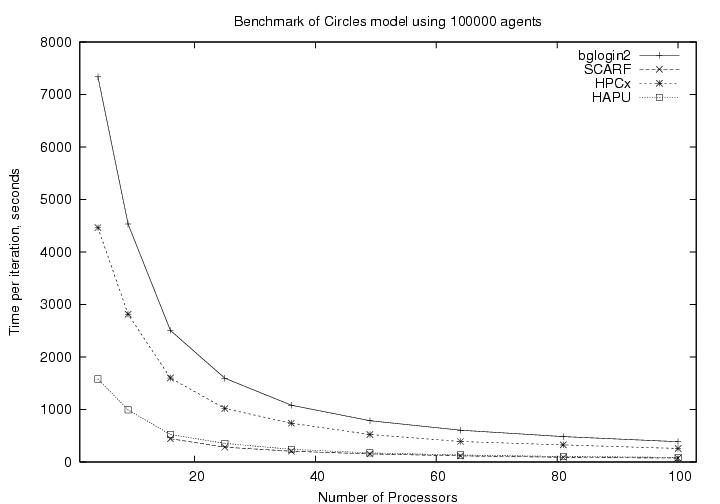
\includegraphics[width=300pt]{Circles-graph.jpg}
 \caption{Graph of iteration times}
 \label{fig:Circles-graph}
\end{figure}

The results indicate that this simulation benefits from using 30 to 50 processors after which the performance benefits flatten. It is interesting to note that this is essentially similar across the range of systems used. The variations between systems being attributed to memory, architecture and communications hardware differences.

\subsection{The C@S Model}
The C@S model was the first economic model to be implemented in FLAME by the EURACE Project.  It is based on work detailed in Delli Gatti \textsl{et al.} \cite{Delli Gatti} where an economy is populated by a finite number of \textsl{firms}, \textsl{workers}/\textsl{consumers} and \textsl{banks}. The acronym C@S stands for \textsl{Complex Adaptive Trivial System}.

This provides an initial economic model for testing FLAME. The EURACE version of C@S contains models for consumption goods, labour services and credit services. The population is a mix of agents: \textsl{Malls}, \textsl{Firms} and \textsl{People}. Each of these has different states and communicates with other agents in the population through 9 message types.

As the agents in the C@S Model have some positional/location data and the communication is localised, the initial distribution of agents to processors, as in the Circles Model, can be based on location. This helps reduce cross-processor communication.

The initial population contained: 20000 firms, 100000 people and 4000 malls (124000 agents in total).

{
\renewcommand{\arraystretch}{1.25}
\begin{table}[ht]
 \centering
  \begin{tabular}{c|cccc}
 Processors &SCARF &HAPU &HPCx  &bglogin2 \\ \hline
4 &2223.86 &3062.12 &- &-       \\
9 &1462.14 &2014.56 &- &-       \\
16 &913.52 &1159.32 &- &4888.57 \\
25 &592.44 &755.84 &2235.92 &3138.71    \\
36 &416.84 &534.62 &1589.53 &2165.96    \\
49 &307.15 &411.32 &1178.06 &1600.83    \\
64 &260.53 &313.39 &910.23 &1218.58     \\
81 &207.25 &261.33 &723.87 &992.43      \\
100 &169.46 &207.52 &601.24 &806.16     \\
 \end{tabular}
 \caption{Execution Times for C@S Model}
 \label{tab:ExecutionTimesForC@S}
\end{table}
}

%\bigskip
\begin{figure}[ht]
 \centering
  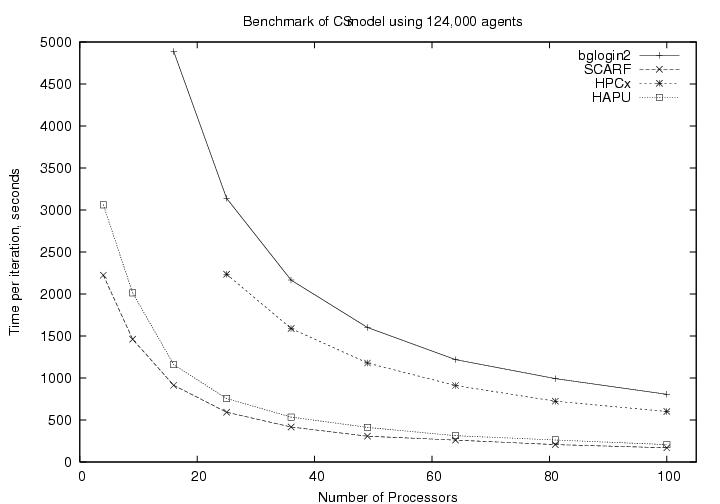
\includegraphics[width=300pt]{C@S2-graph.jpg}
 \caption{Graph of C@S Model execution times}
 \label{fig:C@S-graph}
\end{figure}

The results show a potential reduction of the elapsed time of the simulation when using up to 30 processors.



\subsection{Initial Labour Market}

This model was first model based on the work of the EURACE project. The model represented a very simplified labour market. It contains four agent types: \textit{Firm}, \textit{Household}, \textit{Market Research} and \textit{Eurostat} and 10 message types.

{
\renewcommand{\arraystretch}{1.25}
\begin{table}[ht]
 \centering
  \begin{tabular}{c|cccc}
 Processors &SCARF &HAPU  &HPCx   &bglogin2 \\ \hline
4 &1149.21 &1388.55 &- &7014.64 \\
9 &585.19 &627.45 &2317.21 &3120.96     \\
16 &334.17 &352.51 &1332.30 &1755.93    \\
25 &198.85 &233.35 &841.33 &1129.25     \\
36 &291.00 &160.97 &612.14 &782.70      \\
49 &206.82 &119.66 &449.91 &574.50      \\
64 &90.67 &97.81 &352.29 &440.36        \\
81 &72.51 &74.81 &273.78 &349.31        \\
100 &60.79 &61.34 &218.11 &284.29       \\
 \end{tabular}
 \caption{Execution Times for Labour Market Model}
 \label{tab:ExecutionTimesForLabour}
\end{table}
}
%\bigskip

\begin{figure}[ht]
 \centering
  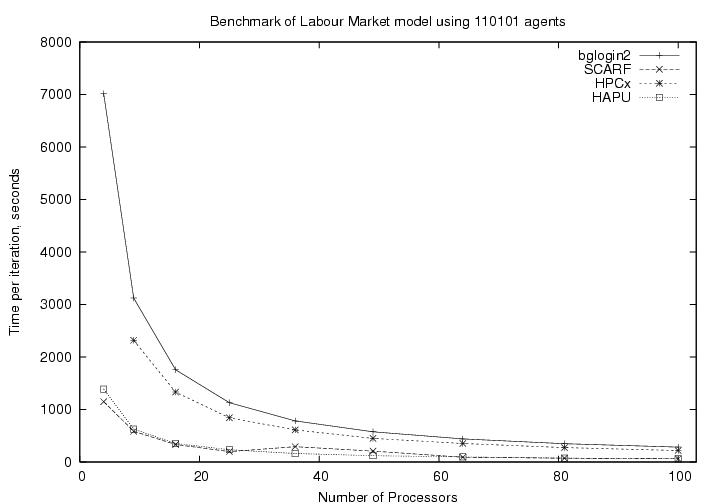
\includegraphics[width=300pt]{Labour2-graph.jpg}
 \caption{Graph of Labour Market Model iteration times}
 \label{fig:Labour-graph1}
\end{figure}

\subsection{Bielefeld Labour Market}

This model is a refinement of the Initial Labour Market. It too contains four agent types, \textit{Firm}, \textit{Household}, \textit{Mall} and \textit{Investment Goods Producer} and has 27 message types.

{
\renewcommand{\arraystretch}{1.25}
\begin{table}[ht]
 \centering
  \begin{tabular}{c|cccc}
 Processors &SCARF &HAPU &HPCx   &bglogin2 \\ \hline
4 &1078.51 &1344.86 &3253.83 &- \\
9 &542.11 &616.52 &1485.97 &-   \\
16 &318.55 &362.18 &847.84 &1173.15     \\
25 &256.06 &231.78 &552.62 &753.00      \\
36 &178.75 &162.90 &386.80 &525.79      \\
49 &119.29 &124.79 &288.37 &390.83      \\
64 &93.39 &99.91 &222.95 &299.56        \\
81 &71.06 &75.00 &179.58 &239.38        \\
100 &65.59 &61.18 &144.97 &194.95       \\
 \end{tabular}
 \caption{Execution Times for Bielefeld Model}
 \label{tab:ExecutionTimesForBielefeld}
\end{table}
}
%\bigskip

\begin{figure}[ht]
 \centering
  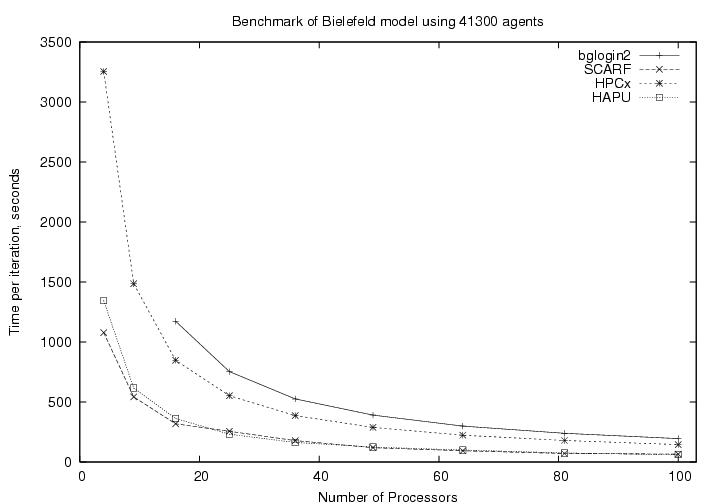
\includegraphics[width=300pt]{Bielefeld2-graph.jpg}
 \caption{Graph of Bielefeld Model iteration times}
 \label{fig:Labour-graph2}
\end{figure}

\subsection{EURACE Models}

During the development of the EURACE Model a number of domain specific models have been developed. These models were then integrated into the EURACE Model. Three domain specific models were developed: Credit Market, Labour Market and Financial Market. Each of these and the combined EURACE Model are the major economic models developed by EURACE. As part of the development of FLAME these models have been used to test the FLAME application generation and the framework infrastructure. In particular they have been very useful in testing the parallel implementation of FLAME. Although the initial agent populations is these models are very small they do encapsulate the full range and complexity of the EURACE model and to that end they are a very useful testing resource.

\begin{table}[ht]
 \centering
  \begin{tabular}{l|ccc}
  Model & Agents & Messages & Population \\\hline
  Financial Market  &    4    &   6       &  1104          \\
  Labour Market   &   7     &    45      &   1236         \\
  Credit Market   &   3     &    12      &   110         \\ 
  EURACE Model    &   9     &    54       &  2029         \\\hline
  \end{tabular}
  \caption{Details of Current EURACE Models}
\end{table}

All these models have been successfully parsed, compile and executed in both serial and parallel on some of our target HPC machines.
\section{Dynamic Load Balancing Overview} %load balancing
\subsection{Dynamic Load Balancing Overview}

The overall aim of parallelising the FLAME framework is to reduce the wall clock time for running a simulation. This relies on efficient parallelisation of communication and keeping the work load balanced between computing nodes. The message board library addresses the first of these and dynamic load balancing addresses the second.

To illustrate the problems in getting load balancing right the diagram in Figure \ref{fig:load_balance_problem} shows agents on two nodes and their communication patterns. The top portion shows an unbalanced number of agents but the frequent communication is internal to each node with only infrequent communication between the nodes. If agents are moved to try to balance the load then frequent communication between nodes is introduced (lower portion of figure) which could mean a large increase in communication time and hence wall clock time. 

This example shows that measurement of communication between nodes must be part of the load balancing algorithm as well as elapsed time for various parts of the framework.

\begin{figure}[h]
 \centering
  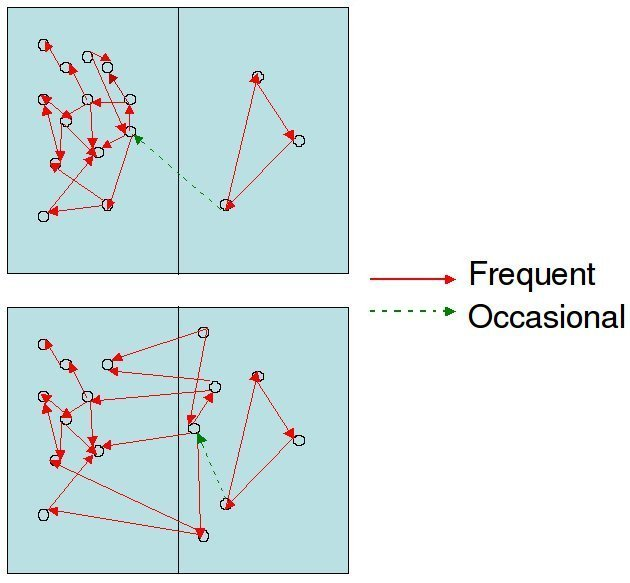
\includegraphics[scale=0.50]{load_balance.jpg}
 \caption{Illustrating some problems of load balancing}
 \label{fig:load_balance_problem}
\end{figure}

This section describes our initial thoughts on dynamic load balancing. The implementation has started with a timer which allows developers to insert timing into any section of FLAME from the framework itself to the user's model functions. It will be timing of different parts of the framework (which includes calls to the user's functions) that provides data for algorithms that seek to balance computational load.

\subsection{The \textit{timer} Package}

Timers will be used to measure the elapsed CPU time for portions of the running code and this data will be used as input to the load balancing strategy used in the FLAME framework. The initial requirements against which the timer package was implemented are given below.

\begin{itemize}
\item Can have multiple timers running simultaneously
\item Timers can be identified individually
\item Functions to start/stop/reset a named timer
\item Function to get elapsed time from a named timer
\item Definition of a set of timers.
\item Functions to get statistics from a set of timer
\item Turn timing on/off during program execution 
\end{itemize}

We have implemented all the functionality for individual timers and a set of unit tests and an example program using the timers. Code is stored under Subversion source code control in the FLAME project on the CCPForge site. 

User documentation is supplied in \cite{TimerAPI}.

\section{The $timer$ Package}%\section{The $timer$ Package}
\label{app:timer-package}
Timers will be used to measure the elapsed CPU time for portions of the running code and this data will be used as input to the load balancing strategy used in the FLAME framework. The initial requirements against which the timer package was implemented are given below.

\begin{itemize}
\item Can have multiple timers running simultaneously
\item Timers can be identified individually
\item Functions to start/stop/reset a named timer
\item Function to get elapsed time from a named timer
\item Definition of a set of timers.
\item Functions to get statistics from a set of timer
\item Turn timing on/off during program execution 
\end{itemize}

We have implemented all the functionality for individual timers and a set of unit tests and an example program using the timers. Code is stored under Subversion source code control in the FLAME project on the CCPForge site. 

User documentation is supplied in \cite{TimerAPI}.

We have demonstrated the use of timers in the simple circles model by timing the work done by agents as the number of partitions over which the agents are distributed increases. The agents were not uniformly distributed in space and so, with geometric partitioning, some partitions will have more agents than others. The time taken by the agents on each node is plotted against the number of agents on the node in Figure \ref{fig:circle_timings} and we can see that there is a direct relation between the number of agents and the work done on each node. From this we can conclude that distributing the agents equally over the nodes will give a good load balance.

There is a cautionary note to be struck however. The timing data for circles has illustrated the problem identified in the overview, namely that naively giving equal numbers of agents to each node without taking into account communication can lead to worse performance. Comparing elapsed time for geometric and round robin for 5 partitions in Figure \ref{fig:timings_problems} shows that the elapsed time increased even though the work done by the agents decreased.

\begin{figure}[h]
 \centering
  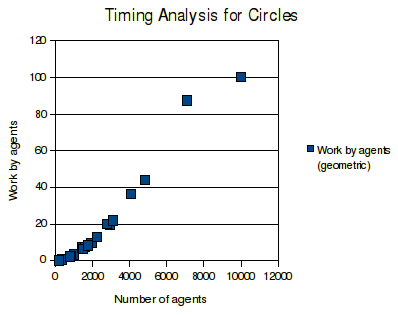
\includegraphics[scale=0.75]{circles-timings.png}
 \caption{Timings results from Circles model}
 \label{fig:circle_timings}
\end{figure}

\begin{figure}[h]
  \hspace{-10mm}
  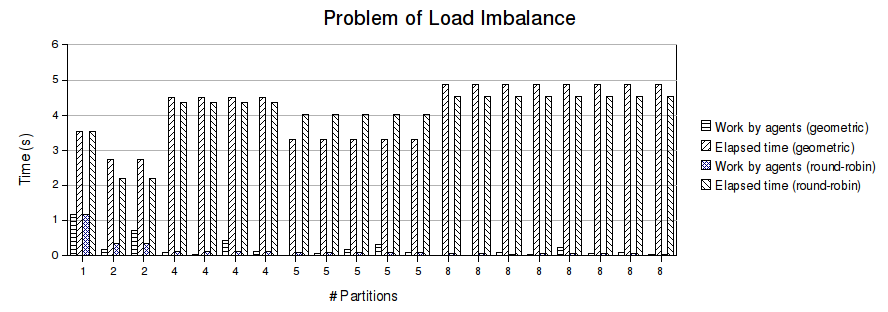
\includegraphics[scale=0.6]{timings-problems.png}
 \caption{Illustration of problems with load balancing with Circles model}
 \label{fig:timings_problems}
\end{figure}

A further example, this time from the full EURACE model, shows the top 5 elapsed times for each iteration for the first 40 iterations: see Figure \ref{fig:timing_example}.

\begin{figure}[h]
  \hspace{-10mm}
  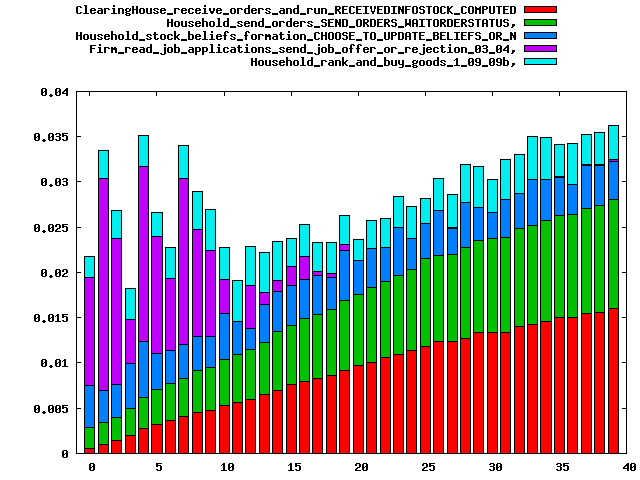
\includegraphics[scale=0.5]{timing_example.png}
 \caption{Example function timing results for EURACE Model}
 \label{fig:timing_example}
\end{figure}

\section{Remote Job Submission}%job submission
\subsection{Introduction}

A job submission system for FLAME jobs has been designed and implemented  so that it is easy to run EURACE on remote (parallel) machines. It will rely on the user knowing details of how to connect to the remote machine and details of the job scheduling software it uses. This data will be stored, in the appropriate format in a machine configuration file. The sequence of steps for job submission was drawn up in discussion with TUBITAK and is as follows:

\begin{enumerate}
 \item \textbf{Check authentication}. Does the user provided information allow a log in to the target machine? Return code for success/failure.
    \item \textbf{Check FLAME version}. Is the required version of FLAME available on the target machine? If not copy files onto target and install. Return code for success/failure of installation or success if installed. Could be some output text to say when FLAME has to be installed.
    \item \textbf{Create a project}. Send the model XMML file and C code. Parse and compile the model. Return code for parse failure/compilation failure/success. Success return code is the project id.
    \item \textbf{Submit job}. Send the 0.xml file(s) and project id. Submit the job according to data in the machine's configuration file. Return code code for success/failure. Success return code is the job id.
    \item \textbf{Query job status}. Send project and job id. Return code pending/done/running/failed.
    \item \textbf{Query status of all jobs in project}. Send project id. Return code is whether data is returned or not. Return text could be {job id, status} for each job.
    \item \textbf{Query status of all jobs in all projects}. Return code is whether data is returned or not. Return text could be {job id, status} for each job.
    \item \textbf{Get results}. Send project and job id. Copy results back and gather if parallel. Return code for success/failure. 
\end{enumerate}

The details for each of these steps are given later.

Connection to remote machines will be via \texttt{ssh} a standard secure connection mechanism which encrypts data between machines, or \texttt{gsissh} a grid-enabled version of ssh (part of Globus \verb+http://www.globus.org+) which requires the user to have a grid (X.509) certificate. The scripts will work best if the user arranges for login authentication without a password. For ssh this means generating a public/private key pair (see the Authentication section of \texttt{ssh} manual and the \texttt{ssh-keygen} manual for details). The public key should be copied to the remote machine and then, using \texttt{ssh-agent} as shown below the operations can be carried out without further authentication.

\begin{verbatim}
# Get the environment variables for ssh-agent
ssh-agent > file
# Set the variables
. ./file
# Add the private key to this session. Will require pass phrase for ssh key
ssh-add
# Run the job submission you want. As an example I have put in a simple ssh
ssh user@remote.machine.ac.uk
# Kill the ssh-agent session
ssh-agent -k	
\end{verbatim}


For gsissh the process is different. The local Grid computing community will have details on obtaining and using a Grid certificate and possibly be able to give advice on installing enough of Globus to use gsissh. It is beyond the scope of this document to go further.

\subsection{Authentication}

This will check whether the user and remote machine data given in the configuration file allow a log in to the remote machine. Comparing the hostname of the remote machine with that in the configuration file will indicate whether the log in was successful or not.

\subsection{Check FLAME}

Check for the xparser executable on the remote machine, assuming that its presence means that necessary libraries (such as the message board library) are therefore present. First look in the \texttt{\$PATH} environment variable and if not found then look in a known directory where a previous check may have installed the parser. If the parser is found then check the version against that version required by the user. If the version is correct the script finishes. 

If the parser is not found or the version is incorrect then the script copies the source for the parser and associated libraries to the remote machine and builds and installs them in a known directory.

\subsection{Create Project}

A project comprises the XMML file and C code for a model and then jobs are added to projects by giving the initial data, number of iterations and number of partitions for a FLAME run. The project is created by giving a directory on the local machine where the XMML and C code files can be found and they are copied to the remote machine. The xparser is run on the copied data and the resulting C code compiled. Errors from the parsing or compilation stages are reported where necessary and when the project has been successfully created it is given a project id that is returned to the user. 

\subsection{Submit Job}

The initial data file is copied to the remote machine and the run initiated for the user defined number of iterations and number of partitions. The job should be assigned to a particular project so the system knows what model is to be run.  Typically large parallel machines use some form of job scheduler to ensure users get a fair share of the machine and details of how to submit jobs to the scheduler should be provided by the user. These details go in the configuration file. When the job is scheduled on the remote machine the script returns a job id for the user to use later in queries.

It is possible to run jobs interactively, that is the script starts the job and waits until it is complete before returning.

\subsection{Query Job Status}

There are a number of variations for job status query, the simplest being querying the status of one job from one project. The information returned to the user will indicate whether the job has finished, is waiting to be started by the job scheduler, is running or has failed. The progress of a job can be monitored by comparing the names of output files (currently named \texttt{node$<$node-id$>$-$<$iteration$>$.xml}) against the number of iterations required for the job.

This basic query can be extended to retrieve the status for all jobs in a project and all jobs in all projects.

\subsection{Get Results}

When a job is complete the results will be left on the remote machine and will need to be copied to the local machine. For a parallel run each node writes its results to separate files, one for each iteration. Current analysis techniques require the results files from each node to be amalgamated into one file for each iteration. There is a script to do this and further scripts based on XSLT (a language for transforming XML documents into other XML documents, see \verb+http://www.w3.org/TR/xslt.html+) can be written to extract information about particular variables of interest.

\subsection{Implementation}

Since the job submission ideas described above require a lot of work with \texttt{ssh/scp} and other command line utilities the job submission system has been implemented as a number of (bash) shell scripts each performing one of the tasks described above. Integration with a GUI which TUBITAK have indicated will be written in Python is simple using the \texttt{os.system} module. The script results can be redirected to a file and the file parsed by the GUI to extract useful information to display to the user.

Data on projects and jobs will be stored in a file on the remote system so that project and job ids will be unique and details about the parameters for a particular job can be retrieved at a later time, e.g.\ for a job status query and retrieving the results. For simplicity this is a text file at present.

\section{FLAME Verification} %\section{FLAME Verification} %\section{FLAME Verification} \input{flameverification}
\label{app:flameverification}
It is important to ensure that applications generated by the FLAME framework execute \textsl{correctly} in both their serial and parallel modes. Because of the stochastic nature of the agent-based approach to modelling it is unrealistic to expect complex simulations to following exactly the solution path although general trends should be similar. However for some simple applications we can expect the serial and parallel implementations to produce exactly the same results throughout the simulation. Such example applications can be used to verify the correctness of both the serial and parallel implementations.

The \textsl{Circles Model} is one such application. The \textsl{Circles} agent is very simple. It has a position in two-dimensional space and a radius of influence. Each agent will react to its neighbours within its interaction radius repulsively. So given a sufficient simulation time the initial distribution of agents will tend to a field of uniformly spaced agents. Each agent has $x$, $y$, $fx$, $fy$ and $radius$ in its memory and has three states: outputdata, inputdata and move. The agents communicate via a single message board, $location$, which holds the agent $id$ and position. Given the simplicity of the agent it is possible to determine the final result of a number of ideal models.

A set of simple test models and problems have been developed based on the \textsl{Circles} agent. Each test has a \texttt{model.xmml} file and a set of initial data (\texttt{0.xml}).
\begin{description}
 \item [Test 1]: Model: single \textsl{Circles} agent type; Initial population of no agents.
 \item [Test 2]: Model: single \textsl{Circles} agent type; Initial population of one agent at (0,0).
	\item [Test 3]: Model: Two \textsl{Circles} agent type; Initial population of agents at (-1,0) and (+,0).
	\item [Test 4]: Model: Four \textsl{Circles} agent type; Initial population of one agent at ($\pm$1,$\pm$1).
	\item [Test 5]: Model: Four \textsl{Circles} agent type; Initial population of one agent at (0,$\pm$1) and ($\pm$1,0).
	\item [Test 6]: Model: Four \textsl{Circles} agent type; Initial population of one agent at random positions.
	\end{description}
In each of these models the expected results can be specified and therefore they provide a very simple check of the implementation.

The \textsl{Circles} agent also provides a good mechanism to check the parallel implementation against the serial. Such is the nature of the model, the positions of the agents at each iteration of the simulation is independent of the order of calculation. As the order of calculation can not be easily prescribed in the parallel simulation we can use this characteristic to test the validity of the parallel implementation against the serial. We would expect to get the identical positions for each agent at every iteration of the simulation.


\label{app:flameverification}
It is important to ensure that applications generated by the FLAME framework execute \textsl{correctly} in both their serial and parallel modes. Because of the stochastic nature of the agent-based approach to modelling it is unrealistic to expect complex simulations to following exactly the solution path although general trends should be similar. However for some simple applications we can expect the serial and parallel implementations to produce exactly the same results throughout the simulation. Such example applications can be used to verify the correctness of both the serial and parallel implementations.

The \textsl{Circles Model} is one such application. The \textsl{Circles} agent is very simple. It has a position in two-dimensional space and a radius of influence. Each agent will react to its neighbours within its interaction radius repulsively. So given a sufficient simulation time the initial distribution of agents will tend to a field of uniformly spaced agents. Each agent has $x$, $y$, $fx$, $fy$ and $radius$ in its memory and has three states: outputdata, inputdata and move. The agents communicate via a single message board, $location$, which holds the agent $id$ and position. Given the simplicity of the agent it is possible to determine the final result of a number of ideal models.

A set of simple test models and problems have been developed based on the \textsl{Circles} agent. Each test has a \texttt{model.xmml} file and a set of initial data (\texttt{0.xml}).
\begin{description}
 \item [Test 1]: Model: single \textsl{Circles} agent type; Initial population of no agents.
 \item [Test 2]: Model: single \textsl{Circles} agent type; Initial population of one agent at (0,0).
	\item [Test 3]: Model: Two \textsl{Circles} agent type; Initial population of agents at (-1,0) and (+,0).
	\item [Test 4]: Model: Four \textsl{Circles} agent type; Initial population of one agent at ($\pm$1,$\pm$1).
	\item [Test 5]: Model: Four \textsl{Circles} agent type; Initial population of one agent at (0,$\pm$1) and ($\pm$1,0).
	\item [Test 6]: Model: Four \textsl{Circles} agent type; Initial population of one agent at random positions.
	\end{description}
In each of these models the expected results can be specified and therefore they provide a very simple check of the implementation.

The \textsl{Circles} agent also provides a good mechanism to check the parallel implementation against the serial. Such is the nature of the model, the positions of the agents at each iteration of the simulation is independent of the order of calculation. As the order of calculation can not be easily prescribed in the parallel simulation we can use this characteristic to test the validity of the parallel implementation against the serial. We would expect to get the identical positions for each agent at every iteration of the simulation.




% End of document
\end{document} 
